\documentclass{article}

\usepackage{amsfonts}
\usepackage{amssymb,amsmath,amsthm}
\usepackage{graphicx}
\usepackage{bm}           % bold math symbols (\boldsymbol)

\usepackage{pstricks}
\usepackage{pstricks-add}
%\usepackage[breaklinks=true]{hyperref}
%\usepackage{breakcites}
\usepackage{microtype}    % melhorias no micro-espaçamento de texto
%\usepackage{minibox}   % para caixa de texto com borda
\usepackage{framed}

\usepackage{algorithm}
\usepackage{algpseudocode}

%%%   PREDEFINITIONS   %%%%%%%%%%%%%%%%%%%%%%%%%%%%%%%%%%%%%%%%%%%%%%%%%%%%%%%%%
\newcommand{\kdtree}{$k$-d~tree}
\newcommand{\bsym}[1]{\boldsymbol{#1}}
\newcommand{\sol}[1]{\boldsymbol{#1}}
\newcommand{\fsol}[1]{f(\sol{#1})}
\newcommand{\np}{m}
\newcommand{\nphard}{$\mathcal{NP}$-Hard}
\newcommand{\missing}[1]{
  \begin{framed}
    {\scriptsize \bf #1}
  \end{framed}
}
\newcommand{\weight}[1]{w(\sol{#1})}
\newcommand{\bigweight}[1]{w\big(\sol{#1}\big)}
\newcommand{\dom}[2]{dom(\sol{#1}, \sol{#2})}
\newcommand{\domk}[2]{dom_k(\sol{#1}, \sol{#2})}
\newcommand{\setIN}{\{1, \ldots, n\}}
\newcommand{\ext}[2]{ext(\sol{#1}, \sol{#2})}
\newcommand{\domLess}[2]{ \sol{#1} \prec \sol{#2} }
%\newcommand{\logicAnd}{ \textrm{ and } }
\newcommand{\logicAnd}{ \land }
\newcommand{\logicOr}{ \lor}
\newcommand{\solSetA}{ Q }
\newcommand{\solSetB}{ R }
\newcommand{\solSett}{ S_* }
\newcommand{\solSet}{ S }
\newcommand{\ord}{\mathcal{O}}
\newcommand{\cb}[2]{cb^{#1}(#2)}  % cost-benefit function

\newtheorem{theorem}{Theorem}

\begin{document}

\title{A fast dynamic programming multi-objective knapsack problem}

\author{
   Marcos Daniel Valad\~ao Baroni\thanks{Research supported by Funda\c c\~ao de Amparo \`a Pesquisa do Esp\'irito Santo.}
   \and
   Fl\'avio Miguel Varej\~ao
}


%%%   OUTLINE   %%%%%%%%%%%%%%%%%%%%%%%%%%%%%%%%%%%%%%%%%%%%%%%%%%%%%%%%%%%%%%%%
% 1. Introduction
%    - The problem and its application
%    - Literature background
%    - The Bazgan algorithm
%    - Our approach
%    - Article structure
% 2. The MOKP
%    - (some definition needed)
%    - Multi-objective problems
% 3. Dyn. Programming Alg. for MOKP
%    - Process overview of DP for MKP
%    - Dom. relations
%    - Application of dom. rel.
% 4. Use of KDTree
%    - (motiuvation: ops. on the algorithms)
%    - The KDTree data structure (...performance issues/dimensions)
%    - Operations
% 5. Experiments
%    - Instances
%    - Results
% 6. Conclusions
%    - (could not achieve bazgan times)


%%%   STRUCTURE %%%%%%%%%%%%%%%%%%%%%%%%%%%%%%%%%%%%%%%%%%%%%%%%%%%%%%%%%%%%%%%%

\maketitle

\begin{abstract}


\begin{resumo}
Resumo...
\vspace{\onelineskip}

\noindent
\textbf{Palavras Chave}:
Multi-objective Knapsack Problem,
Metaheuristic,
Shuffled Complex Evolution,
Multi-dimensional indexing
\end{resumo}

\begin{resumo}[Abstract]
 \begin{otherlanguage*}{english}
Many real applications like project selection, capital budgeting and cutting stock involves optimizing multiple objectives that are usually conflicting and can be modelled as a multi-objective knapsack problem (MOKP).
Unlike the single-objective case, the MOKP is considered a NP-Hard problem with
considerable intractability.
This work propose a hybrid heuristic for the MOKP based on the
shuffled complex evolution algorithm.
A multi-dimensional indexing strategy for handling large amount of intermediate
solutions are proposed as an optimization, which yields considerable
efficiency, especially on cases with more than two objectives.
A series of computational experiments show the applicability of the proposal
to several types of instances.

\noindent
\textbf{Keywords}:
Multi-objective Knapsack Problem,
Metaheuristic,
Shuffled Complex Evolution,
Multi-dimensional indexing
\end{otherlanguage*}
\end{resumo}

% Falar brevemente sobre o MOKP
% Falar brevemente sore a estratégia de indexação
% Resumir os resultados obtidos

\missingt{
Observar as 5 regras:\\
1. A general statement introduciong the broad reserach area of the particular topic being investigated;\\
2. An explanation of the specific problem (difficulty, obstavle, challange) to be solved;\\
3. A review of existing or standard solutions to this problem and their limitations;\\
4. An outline of the proposed new solution;\\
5. A summary of how the solution was evaluated and what the outcomes of the evaluation were.
}


\end{abstract}

\section{Introduction}
\label{sec:intro}
% THE MOKP Problem

% MO problems
\begin{frame}
\frametitle{Multi-objective problems}
\textbf{Multi-objective problems} are optimization problems involving optimizing multiple criteria.
\pause
\begin{itemize}
  \item{ Usually conflicting criterias; }\pause
  \item{ A set of \textit{optimal} (non-dominated) solutions; } \pause
  \item{ Models many real applications. }
\end{itemize}
\vfill
\end{frame}

% MOKP
\begin{frame}
\frametitle{The multi-dimensional knapsack problem}
The \textbf{multi-dimensional knapsack problem} (MOKP)
is one of the most important multi-objective problems.
\pause
\begin{itemize}
  \item{ Is a generalization of the $0-1$ knapsack problem (\nphard); }\pause
  \item{ Models project selection, capital budgeting, cargo loading, flow shop scheduling and others;} \pause
  \item{ Models many real applications; }
\end{itemize}
\end{frame}

% Motivation
\begin{frame}
\frametitle{Motivation}
Several exact approaches have been proposed in the literature for
solving the MOKP. \\ \pause
\vfill
However no effective exact method for large MOKP, expecially with
more than two objectives. \\ \pause
\vfill
Even for the bi-objective case, some medium sized instances
has shown to be hard to solve exactly. \\ \pause
\vfill
This reason motivates the development of heuristic methods.
\vfill
\end{frame}

% The Proposal
\begin{frame}
\frametitle{Proposal}
This work proposes the development of a heuristic for the MOKP
based on an evolutionary algorithm called shuffled complex evolution (SCE).
\\ \medskip \pause
As a performance improvement for the approach,
a multi-dimensional indexing strategy
will be used for handling the large amount of solutions.
\\ \medskip \pause
The SCE has been successfully used for solving optimization problems, among then,
the multi-dimensional knapsack problem (MKP) (also a contribution of this work).
\end{frame}

% Contributions and Publications
\begin{frame}
\frametitle{Contributions and Publications}\pause
\begin{enumerate}
\item{
\textbf{Efficient indexing strategy for MOKP solutions:} \pause
\begin{itemize}
 \item[{\tiny$\bullet$}] { BARONI, M. D. V; VAREJ\~AO, F. M. Multi-dimensional indexing on dynamic programming for multi-objective knapsack problem. \textit{International Transactions in Operational Research}, Wiley Online Library, 2017, Submitted. }
\end{itemize}
} \pause
\medskip
\item{
\textbf{A SCE algorithm for the MKP:} \pause
\begin{itemize}
  \item[{\tiny$\bullet$}] { BARONI, M. D. V; VAREJ\~AO, F. M. A shuffled complex evolution algorithm
  for the multidimensional knapsack problem. In: \textit{Progress in Pattern Recognition, Image Analysis, Computer Vision, and Applications.} [S.l.]: Springer, 2015. p. 768-775. }
  \pause
 \item[{\tiny$\bullet$}] { BARONI, M. D. V; VAREJ\~AO, F. M. A shuffled complex evolution algorithm
  for the multidimensional knapsack problem using core concept. In: IEEE. \textit{Evolutionary Computation (CEC), 2016 IEEE Congress on.} [S.l.], 2016 p. 2718-2723. }
\end{itemize}
} \pause
\medskip
\item{
\textbf{Hybrid heuristic for MOKP:} \pause
\begin{itemize}
 \item[{\tiny$\bullet$}] { BARONI, M. D. V; VAREJ\~AO, F. M. An efficient shuffled complex evolution algorithm for the multi-objective knapsack problem. In: IEEE \textit{Evolutionary Computation (CEC), 2018 IEEE Congress on.} [S.l.], 2018, In Preparation }
\end{itemize}
}
\end{enumerate}
\end{frame}


\section{The Multiobjective Knapsack Problem}
\label{sec:mokp}

%%% Definição de problema multi-objectivo

Em problemas reais é comum a existência de situações em que deseja-se otimizar
mais de um objetivo os quais, geralmente, são conflitantes.
Estes problemas são chamados multiobjetivos e tipicamente não possuem
uma solução sendo a melhor em todos os objetivos, mas as possuem várias
soluções de interesse chamadas \emph{soluções eficientes}.

Um problema de otimização multi-objetivo com $\np$ objetivos pode ser descrito como uma
função vetorial $f(x) = \big(f_1(x), \ldots, f_p(x)\big)$
para a qual deseja-se encontrar um vetor $x \in X$
que maximize simultaneamente as $\np$ funções objetivo.
Formalmente:
\begin{align*}
  \text{max} ~ f(x) &=
    \big(f_1(x)
    ,f_2(x)
    ,\ldots
    ,f_{\np}(x)\big) \\
  \text{sujeito a} ~ x & \in X
\end{align*}

\begin{mydef}[Dominância, Eficiência e \paretoset]
Considere um problema de otimização multi-objetivo.
Diz-se que uma solução $x \in X$
\emph{domina} uma solução $y \in X$, denotado por $\text{dom}(x, y)$
se, e somente se, $x$ é ao menos tão boa quanto
$y$ em todos os objetivos e melhor que $y$ em ao menos um dos objetivos.
Formalmente:
\begin{displaymath}
    \text{dom}(x, y) = \left\{
      \begin{array}{l}
          \forall i \in \{1, 2, \ldots, \np\}: f_i(x) \geq f_i(y) ~\text{e}\\
          \exists j \in \{1, 2, \ldots, \np\}: f_j(x) > f_j(y)
  \end{array} \right.
\end{displaymath}
Uma solução $x \in X$ é dita \emph{eficiente}, denotado por $\text{eff}(x)$,
se, e somente se, $x$ não é dominada por nenhuma outra solução pertencente a $X$.
Formalmente:
\begin{displaymath}
  eff(x) \iff \nexists \big(y \in X \wedge dom(y, x) \big)
\end{displaymath}
O conjunto de todas as soluções eficientes de um problema multi-objetivo,
denotado por $Par(X)$, é chamado de \emph{\paretoset{}} ou \emph{\paretosetII{}}.
Formalmente:
\begin{displaymath}
  Par(X) = \{ x \in X \;|\; \text{eff}(x)\}
\end{displaymath}
\end{mydef}

Resolver um problema multi-objetivo consiste em determinar seu \paretoset{}.
Este conceito foi primeiramente elaborado por Vilfredo Pareto em 1896, que
enunciou a relação Pareto-Ótima que diz: ``não é possível melhorar uma característica
do problema sem piorar outra'', o que caracteriza a relação conflitante entre os
objetivos na otimização multi-objetivo.

Na Figura~\ref{fig:dom-def} ilustra o conceito de dominância.
A solução marcada domina todas as soluções existentes na área hachurada.
As soluções em destacadas na Figura~\ref{fig:eff-def} formam um \paretoset por
dominarem sobre todas as outras soluções.

\begin{figure}
    \centering
    \begin{subfigure}[t]{0.3\textwidth}
        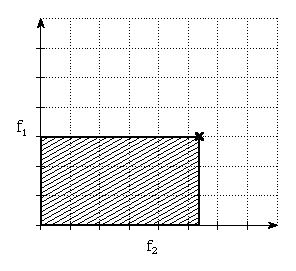
\includegraphics[width=\textwidth]{img/mokp/dom-def}
        \caption{Região de dominância de uma solução.}
        \label{fig:dom-def}
    \end{subfigure}
    \qquad
    \begin{subfigure}[t]{0.3\textwidth}
        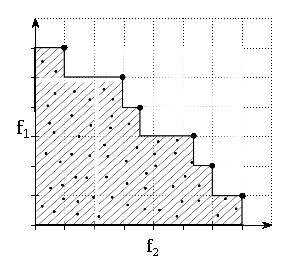
\includegraphics[width=\textwidth]{img/mokp/pareto-def}
        \caption{Exemplo de \paretoset.}
        \label{fig:eff-def}
    \end{subfigure}
    \caption{Exemplos de solução dominante e \paretoset.}
    \label{fig:mo-defs}
\end{figure}

%%% Intro ao MOKP

Um dos problemas multiobjetivos mais importantes da literatura
é o problema da mochila multiobjetivo (\mokp{}).
Muitas problemas reais podem ser modelados como uma instância do \mokp{}
como seleção de projetos~\cite{teng1996multiobjective},
orçamento de capital~\cite{rosenblatt1989generating},
carregamento de carga~\cite{teng1996multiobjective}
e planejamento de estoque~\cite{ishibuchi2015behavior}.

\missing{Comentar sobre a dificuldade de problemas MObj.
Exploão do pareto com o aumento da quantidade de objectivos.
Poucos métodos extados eficientes, geralmente utiliza-se métodos heurísticos.}

%%%%%%%%%%%%%%%%%%%%%%%%%
%%% Definição do MOKP %%%
%%%%%%%%%%%%%%%%%%%%%%%%%
O problema da mochila multi-objetivo pode ser descrito como uma função vetorial
$f$ que mapeia uma variável de decisão (solução) a uma tupla de $\np$ valores
(objetivos).
Formalmente:
\begin{align*}
  \text{max} ~ \sol{y} &= f(\sol{x}) =
    \big(f_1(\sol{x})
    ,f_2(\sol{x})
    ,\ldots
    ,f_{\np}(\sol{x})\big) \\
  \text{sujeito a} ~ \sol{x} & \in X
\end{align*}
onde $\sol{x}$ é a \emph{variável de decisão}, $X$ denota o conjunto de
soluções viáveis e $\sol{y}$ representa o \emph{vetor de objetivos} para os quais
deseja-se maximizar.

Vale resaltar que o tamanho do \paretoset para o problema em questão
tende a crescer rapidamente com o tamanho do problema, especialmente com o
número de objetivos.

Uma instância de um problema da mochila multi-objetivo (\mokp{}) com $\np$
objetivos consiste em uma capacidade inteira $W >0$ e $n$ itens.
Cada item $i$ possui um peso inteiro positivo $w_i$ e $\np$ lucros inteiros
$p_i^1, p_i^2, \ldots, p_{i}^{\np}$ não negativos.
O lucro $p_i^k$ representa a contribuição do $i$-ésimo item
para com o $k$-ésimo objetivo.
Uma solução é representada por um conjunto $\sol{x} \subseteq \{1, \ldots, n\}$
contendo os índices dos itens incluídos na mochila.
Uma solução é viável se o peso total incluído na mochila não ultrapassa
a capacidade da mochila.
Formalmente a definição do problema é a seguinte:
\begin{align*}
  \text{max   } & f(x) =
    \big(f_1(x) ,f_2(x) ,\ldots ,f_{\np}(x)\big) \\
  \text{subject to   } & w(x) \leq W \\
  & x \in \{0, 1\}^n\\
  \text{where} \phantom{mmmmm} \\
  %I_n &= \{1, \ldots, n\}\\
  f_j(x) &= \sum_{i = 1}^n p^j_i x_i \quad j = 1, \ldots, \np\\
  w(x) &= \sum_{i = 1}^n w_i x_i
\end{align*}

O \mokp{} é considerado um problema \nphard{} visto set uma generalização
do bem conhecido problema da mochila $0-1$, para o qual $\np = 1$.
É consideravelmente difícil determinar o \paretoset para um \mokp{},
especialmente para vários objetivos.
Até mesmo para casos bi-objetivos, problemas pequenos podem se apresentar
intratáveis.
Por este motivo interessa-se no desenvolvimento de métodos eficientes
para manipular uma grande quantidade de soluções, o que pode eventualmente
trazer tratabilidade a instâncias antes intratáveis.

A literatura contém várias propostas para resolver o \mokp{} de forma exata.
Porém, nenhum método tem provado ser eficiente para grande instâncias
com mais de dois objetivos.
Mesmo para problemas bi-objetivo, algumas instâncias de tamanho considerado
médio têm aprestando difculdades na determinação da solução exata, o que
tem motivado o desenvolvimento de métodos heurísticas que buscam determinar
um \paretoset aproximado em tempo computacional razoável.


\section{The Dynamic Programming algorithm}
\label{sec:progdyn}
% Breve resumo sobre métodos de programação dynamica
% Explicação overview do método para o MOKP
% - Process overview of DP for MKP
% - Dom. relations
% - Application of dom. rel.
\cite{bazgan2009}


% Basic simple Dynamic Programming
% Nemhauser-Ullmann algorithm



\section{The use of \kdtree{}}
\label{sec:kdtree}
% Histórico da kdtree: 
%  - primeira proposta. 
%  - Objetivo. Eficientcia
%  - Teste de colisão, pertinencia e amplitude
The \kdtree{} is a type of binary search tree for indexing multidimenstional
data with simple construction and low space usage.
Despite its simplicity it efficiently supports operations like nearest
neighbour search and range search~\cite{bentley1975} and is widely used on
spacial geometry algorithms~\cite{preparata2012computational, guttman1984r}, 
clustering algorithms~\cite{kanungo2002efficient, indyk1998approximate}
and ~\cite{owens2007survey}

% Utilizacao:
%  - objetos espaciais 2D/3D):
%  - renderizacao

% Vantagens sobre outras estruturas (quad-tree, etc):
%  - menor sensibilidade a distribuicao tendensiosa.
Its advantages.

% Discussao sobre eficiencia
%  - máximo de dimensoes ( |n| >> 2^dim )
Efficiency notes.

% Estrutura e Operacoes:
%  - estrutura de indexacão
%  - Insercao
%  - range-search
Its operations...

% Utilizacao no Algoritmo
% Possibilidade de utilizacao no processo de range seaarch, ao buscar uma
% solucao dominante.
Use on the algorithm.

% Explicacão da indexacão das solucoes e da funcao de range.
Indexing the solutions and range operations.

% Mencionar que esta proposta de indexacao viabiliza a aplicacão do algoritmo em problemas
% com maiores dimensões.
Tends to increase the feasibility on problems with higher dimensions.


\section{Computational experiments}
\label{sec:exp}
- Base de dados utilizaca \\
- Parametros dos algoritmos \\
- Análise dos resultados (comparação)


\section{Conclusions and future remarks}
\label{sec:conc}
- Conclusões dos resultados \\
- Trabalhos futuros \\


\bibliographystyle{plain}
\bibliography{src/refs}

\end{document}
